\documentclass[conference, compsoc]{IEEEtran}
\IEEEoverridecommandlockouts
\usepackage[numbers]{natbib}
\usepackage[hyphens]{url}
\usepackage{booktabs}
\usepackage{tabularx}
\usepackage{amsmath,amssymb,amsfonts}
\usepackage{algorithmic}
\usepackage{graphicx}
\usepackage{textcomp}
\usepackage{xcolor}
\def\BibTeX{
    {\rm B\kern-.05em{\sc i\kern-.025em b}\kern-.08em
    T\kern-.1667em\lower.7ex\hbox{E}\kern-.125emX}
}

\begin{document}

\title{Predicting Media Memorability Using Visual Features}

\author{
    \IEEEauthorblockN{Zhenshuo Chen}
    \IEEEauthorblockA{
        \textit{School of Computing} \\
        \textit{Dublin City University} \\
        Dublin, Ireland \\
        chenzs108@outlook.com
    }
}

\maketitle

\begin{abstract}
Nowadays, the number of videos is increasing rapidly. Understanding what makes a video memorable would be helpful for advertising, education, etc.
In this paper, I perform short-term and long-term video memorability predictions, which were proposed in MediaEval 2018.
Five regression models,
including Linear, K-Nearest Neighbors, Support Vector, Random Forest and AdaBoost,
are tested using three visual features:
the final classification layer of the 3D Convolutional Neural Network, Histogram of Motion Pattern and Local Binary Pattern.
The models are evaluated using Spearman's correlation coefficients.
Finally, Random Forest gets the best results both for short-term and long-term predictions.
\end{abstract}

\begin{IEEEkeywords}
Media Memorability, C3D, HMP, LBP, Linear Regression, KNN, Random Forest, SVR, AdaBoost
\end{IEEEkeywords}


\section{INTRODUCTION}
Media Memorability Prediction is a part of MediaEval 2018 Benchmarking Initiative for Multimedia Evaluation
and the purpose of this task is to automatically predict the memorability of multimedia content such as movie clips.
As the number of videos is increasing rapidly every day, understanding what makes a video memorable has a very broad range of applications in advertising, education and entertainment areas.
The detail of the task is introduced in \cite{DBLP:journals/corr/abs-1807-01052}.

6000 videos are provided to participants as a training set with different pre-computed features.
Each video also has two memorability scores calculated from the short-term and long-term memorability tests as ground truth.
In this paper, I used the final classification layer of 3D Convolutional Neural Networks (C3D) \cite{DBLP:journals/corr/TranBFTP14}, Histogram of Motion Patterns (HMP) \cite{6116516}, {Local Binary Patterns (LBP) \cite{572934} and their combinations as features,
training models with Linear Regression, $K$-Nearest Neighbors Regression, Support Vector Regression, Random Forest Regression and AdaBoost Regression.
The models were evaluated using the Spearman's correlation coefficient.
Finally, a test set containing 2000 videos is provided for memorability predictions.

In my analysis, Random Forest Regression had the highest Spearman's scores both for short-term and long-term predictions.
But the features were different.
For short-term predictions, I used the combination of C3D and HMP.
While for long-term predictions, the best feature was the combination of C3D and LBP.
The detailed analysis and source code are available on my GitHub\footnote{https://github.com/czs108/Media-Memorability-Prediction}.


\section{RELATED WORK}
\citeauthor{10.1145/3206025.3206056} \cite{10.1145/3206025.3206056} proposed a new protocol measuring very long-term memory performances.
They investigated various kinds of audio and visual features,
including low-level characteristics, emotional and semantic features.
\citeauthor{DBLP:journals/corr/ShekharSSKS17} \cite{DBLP:journals/corr/ShekharSSKS17} explored semantic description, saliency and color descriptors.
But in their experiment, participants were asked textual recall questions instead of the full video being shown again.
They found that image memorability alone was not sufficient to explain the memorability of sub-shots.

\citeauthor{Gupta2018LinearMF} \cite{Gupta2018LinearMF} trained models over features provided by \cite{DBLP:journals/corr/abs-1807-01052},
including visual features and video captions.
The key findings were that models based on video captions outperform models trained on visual features,
and models based on high-level representations learned by Convolutional Neural Networks outperform both models based on visual features and captions.
Reference \cite{RajSingh-1994} is also about MediaEval 2018.
\citeauthor{RajSingh-1994} trained Random Forest, Support Vector Regression and Recurrent Neural Network with C3D, HMP and video captions.
The best model was Random Forest with captions.
And he observed that the videos with high memorability scores had outdoor items like the sky, sea, sun, etc.


\section{APPROACH}
This section describes feature selection and model training.

\subsection{Features}
There were three visual features and their combinations used in my experiments.

\begin{itemize}
    \item C3D: C3D was extracted from the output of the final classification layer of the C3D model, a 3D Convolutional Network proposed for generic video analysis.
    For each video, there is a single list of numbers on one line.
    The dimension is 101.

    \item HMP: It is a single list of pairs of numbers with format \verb|bin:number| on one line for each video.
    The dimension is 6075.

    \item LBP: Unlike the previous two features, LBP was extracted on three key-frames, the first (0), one-third (56) and two-thirds (112), on each video.
    For each frame, it is a single list of numbers on one line, calculated for patches of $8 \times 15$ pixels.
    The dimension depends on the image size.
\end{itemize}

Their combinations include C3D + HMP, C3D + LBP and HMP + LBP.

\subsection{Data Preprocessing}
C3D and HMP are related to the whole video so that they can be directly loaded. In contrast, LBP is corresponding to frames.
To generate a single LBP value for a video, I combined the number lists from three key-frames as a long vector as below.

\begin{equation*}
    \bigl[v_{0}^{0},\, v_{1}^{0},\, \cdots,\, v_{121}^{0},\, v_{0}^{56},\, v_{1}^{56},\, \cdots,\, v_{121}^{56},\, v_{0}^{112},\, v_{1}^{112},\, \cdots,\, v_{121}^{112}\bigr]
\end{equation*}

Where $v_{i}^{j}$ is the $i$th value from the $j$th frame. And 122 is the largest LBP dimension in the training set.

\subsection{Models}
Five models were trained with all features,
including Linear Regression, $K$-Nearest Neighbors Regression, Support Vector Regression, Random Forest Regression and AdaBoost Regression.
The mean of five Spearman's correlation coefficient scores were recorded using 5-fold cross-validation for each short-term and long-term memorability test.
All models were imported from \verb|scikit-learn| library.

\begin{itemize}
    \item Linear Regression: It fits a linear model to minimize the residual sum of squares between targets and predicted values.
    The implementation class is \verb|linear_model.LinearRegression|.

    \item $K$-Nearest Neighbors Regression: It predicts a value based on the $k$ nearest neighbors' mean in the training set.
    The implementation class is \verb|neighbors.KNeighborsRegressor| and its default $k$ is 5.

    \item Support Vector Regression: It is derived from Support Vector Classification.
    It also depends on only a subset of training samples because the cost function will ignore samples whose prediction is close to their target.
    The implementation class is \verb|svm.SVR|.

    \item Random Forest Regression:
    It is an ensemble model made from many decision trees trained on various subsets of samples and uses averaging to improve the predictive accuracy and control over-fitting.
    The implementation class is \verb|ensemble.RandomForestRegressor|.

    \item AdaBoost Regression: Like Random Forest, AdaBoost Regression is also an ensemble model.
    It first fits a regressor on the original dataset and then fits additional copies of the regressor on the same dataset
    but where the weights of instances are adjusted according to the error of the current prediction.
    The implementation class is \verb|ensemble.AdaBoostRegressor|.
\end{itemize}


\section{RESULTS}

\subsection{Memorability Distribution for Development Set}
From Fig.~\ref{fig:dev-set-memo-distribution}, we can see that the long-term memorability scores are relatively less and more variant than the short-term.

\begin{figure}[htbp]
    \centerline{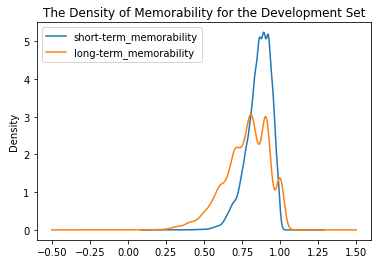
\includegraphics[width=\linewidth]{figures/dev-set-memo-distribution.png}}
    \caption{Memorability distribution for the development set}
    \label{fig:dev-set-memo-distribution}
\end{figure}

\subsection{Short-term Prediction}
Table.~\ref{tbl:short-spearman-scores} and Fig.~\ref{fig:short-spearman-scores} show Spearman's scores for short-term predictions.
The best combination was Random Forest with C3D + HMP. Its Spearman's score of 5-fold cross-validation was $0.334$.
Random Forest also had better performance than other models for each feature.

\begin{table}[htbp]
    \caption{Spearman's scores for short-term predictions}
    \begin{center}
        \begin{tabularx}{\linewidth}{c*5{>{\centering\arraybackslash}X}}
            \toprule
            Feature & Linear & $K$-Nearest & Support Vector & Random Forest & AdaBoost \\
            \midrule
            C3D & $0.276$ & $0.183$ & $0.248$ & $0.304$ & $0.257$ \\
            HMP & $-0.007$ & $0.199$ & $0.278$ & $0.295$ & $0.244$ \\
            LBP & $0.181$ & $0.121$ & $0.250$ & $0.279$ & $0.190$ \\
            C3D + LBP & $0.236$ & $0.219$ & $0.264$ & $0.316$ & $0.260$ \\
            C3D + HMP & $0.007$ & $0.199$ & $0.292$ & $0.334$ & $0.269$ \\
            LBP + HMP & $-0.007$ & $0.222$ & $0.290$ & $0.325$ & $0.259$ \\
            \bottomrule
        \end{tabularx}
    \end{center}
    \label{tbl:short-spearman-scores}
\end{table}

\begin{figure}[htbp]
    \centerline{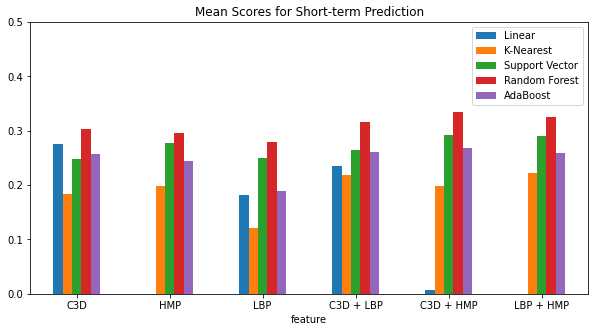
\includegraphics[width=\linewidth]{figures/short-spearman-scores.png}}
    \caption{Spearman's scores for short-term predictions}
    \label{fig:short-spearman-scores}
\end{figure}

The performance of Linear and $K$-Nearest Neighbors Regression highly depended on feature selection.
If the feature contained HMP, Linear Regression's Spearman's scores were almost equal to zero and significantly less than $K$-Nearest Neighbors.
Otherwise, it performed relatively well and better than $K$-Nearest Neighbors.
Overall, Linear Regression was the most unstable model.

Support Vector and AdaBoost Regression got the second and third highest Spearman's scores in most predictions.

\subsection{Long-term Prediction}
Table.~\ref{tbl:long-spearman-scores} and Fig.~\ref{fig:long-spearman-scores} show Spearman's scores for long-term predictions.
All models' long-term Spearman's scores were much less than their short-term scores.
The best model for long-term predictions was also Random Forest, but the feature was C3D + LBP.
Its Spearman's score of 5-fold cross-validation was $0.144$.

\begin{table}[htbp]
    \caption{Spearman's scores for long-term predictions}
    \begin{center}
        \begin{tabularx}{\linewidth}{c*5{>{\centering\arraybackslash}X}}
            \toprule
            Feature & Linear & $K$-Nearest & Support Vector & Random Forest & AdaBoost \\
            \midrule
            C3D & $0.114$ & $0.064$ & $0.093$ & $0.130$ & $0.113$ \\
            HMP & $-0.008$ & $0.060$ & $0.111$ & $0.114$ & $0.079$ \\
            LBP & $0.057$ & $0.038$ & $0.078$ & $0.107$ & $0.066$ \\
            C3D + LBP & $0.082$ & $0.033$ & $0.094$ & $0.144$ & $0.107$ \\
            C3D + HMP & $-0.007$ & $0.064$ & $0.114$ & $0.133$ & $0.090$ \\
            LBP + HMP & $-0.005$ & $0.044$ & $0.112$ & $0.114$ & $0.079$ \\
            \bottomrule
        \end{tabularx}
    \end{center}
    \label{tbl:long-spearman-scores}
\end{table}

\begin{figure}[htbp]
    \centerline{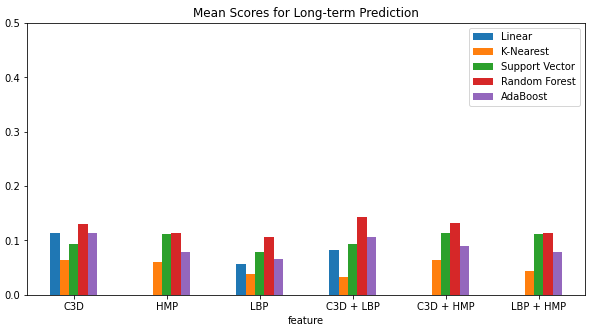
\includegraphics[width=\linewidth]{figures/long-spearman-scores.png}}
    \caption{Spearman's scores for long-term predictions}
    \label{fig:long-spearman-scores}
\end{figure}

The comparison of Linear and $K$-Nearest Neighbors Regression was the same as short-term predictions.
HMP caused severe negative impacts on Linear Regression.

In long-term predictions, Support Vector and Random Forest Regression had similar performance if the feature contained HMP.
For example, when the feature was only HMP, their Spearman's scores were $0.111$ and $0.114$, respectively.
When the feature was LBP + HMP, their Spearman's scores were $0.112$ and $0.114$.
This relation was not so evident in short-term predictions.

\subsection{Predicted Memorability Distribution for Test Set}
After training predictors using suitable models and features on the entire development set, I used them to predict the test set's memorability scores.
Their distribution is shown in Fig.~\ref{fig:test-set-memo-distribution}.

\begin{figure}[htbp]
    \centerline{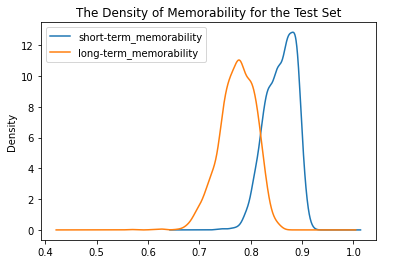
\includegraphics[width=\linewidth]{figures/test-set-memo-distribution.png}}
    \caption{Predicted memorability distribution for the test set}
    \label{fig:test-set-memo-distribution}
\end{figure}


\section{FEATURE ANALYSIS}
This section contains the analysis of the features used by short-term and long-term predictions.

\subsection{Short-term Prediction}
The best model and feature used by short-term predictions were Random Forest and C3D + HMP.
Fig.~\ref{fig:c3d-short-importance} and Fig.~\ref{fig:hmp-short-importance} show the importance of these two features.
The importance values were from \verb|feature_importances_| property of \verb|ensemble.RandomForestRegressor| class.
It is clear that the 21st dimension of C3D is absolutely the most important value for short-term predictions and HMP does not provide much help.

\begin{figure}[htbp]
    \centerline{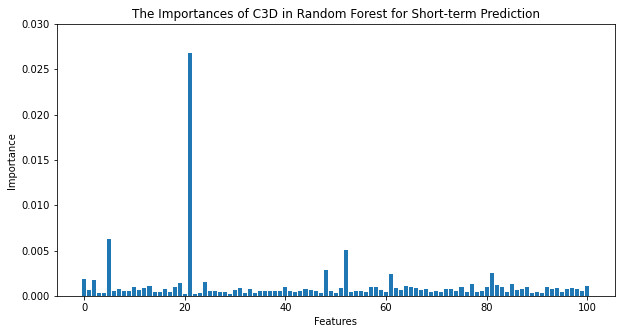
\includegraphics[width=\linewidth]{figures/c3d-short-importance.png}}
    \caption{C3D importance for short-term predictions}
    \label{fig:c3d-short-importance}
\end{figure}

\begin{figure}[htbp]
    \centerline{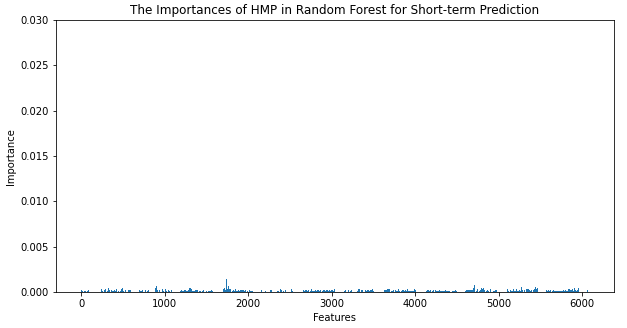
\includegraphics[width=\linewidth]{figures/hmp-short-importance.png}}
    \caption{HMP importance for short-term predictions}
    \label{fig:hmp-short-importance}
\end{figure}

Fig.~\ref{fig:c3d-and-short-memo-distribution} shows the distribution of short-term memorability and C3D's 21st value for the development set.
There is no obvious relation between them.

\begin{figure}[htbp]
    \centerline{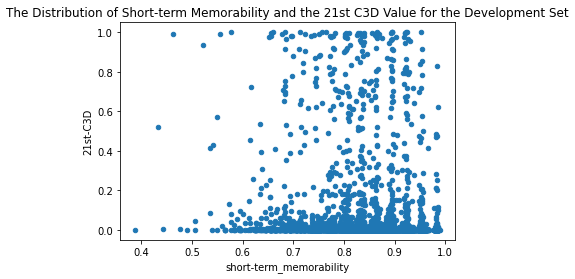
\includegraphics[width=\linewidth]{figures/c3d-and-short-memo-distribution.png}}
    \caption{Distribution of short-term memorability and C3D's 21st value for the development set}
    \label{fig:c3d-and-short-memo-distribution}
\end{figure}

\subsection{Long-term Prediction}
The best model and feature for long-term predictions were Random Forest and C3D + LBP.
Fig.~\ref{fig:c3d-long-importance} and Fig.~\ref{fig:lbp-long-importance} show each feature's importance.
Compared with the feature components used by short-term predictions, the importance of C3D and LBP for long-term predictions is more balanced.
For LBP, considering that an LBP vector was combined from three key-frames, we can see that the values at the beginning, middle and end of a frame are more important than others.

\begin{figure}[htbp]
    \centerline{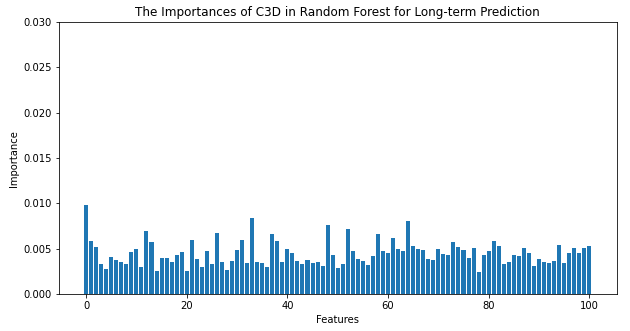
\includegraphics[width=\linewidth]{figures/c3d-long-importance.png}}
    \caption{C3D importance for long-term predictions}
    \label{fig:c3d-long-importance}
\end{figure}

\begin{figure}[htbp]
    \centerline{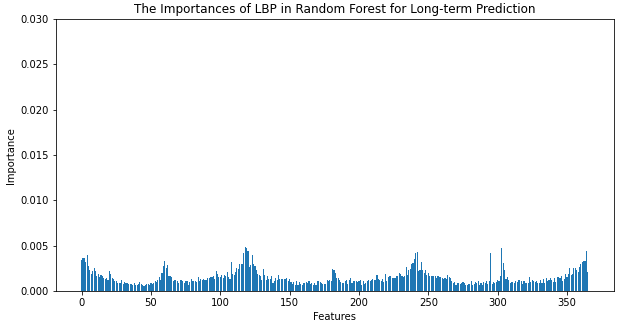
\includegraphics[width=\linewidth]{figures/lbp-long-importance.png}}
    \caption{LBP importance for long-term predictions}
    \label{fig:lbp-long-importance}
\end{figure}

Fig.~\ref{fig:lbp-long-importance-for-a-frame} is a heat map showing LBP importance of the first key-frame.
The resolution would be different for each video.
In general, the most useful values are mainly located at the top, middle and bottom of a frame.

\begin{figure}[htbp]
    \centerline{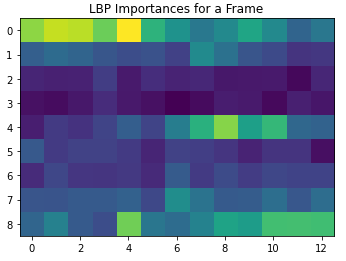
\includegraphics[width=\linewidth]{figures/lbp-long-importance-for-a-frame.png}}
    \caption{LBP importance of the first frame for long-term predictions}
    \label{fig:lbp-long-importance-for-a-frame}
\end{figure}

There are eight heat maps in Fig.~\ref{fig:high-long-memo-lbp} and Fig.~\ref{fig:low-long-memo-lbp}.
The four heat maps in Fig.~\ref{fig:high-long-memo-lbp} show the first key-frame's LBP values of the four videos with the highest long-term memorability scores.
And Fig.~\ref{fig:low-long-memo-lbp} shows the same feature of the four videos having the lowest scores.
It seems that the most memorable videos tend to have large LBP values at the middle of a frame.

\begin{figure}[htbp]
    \centerline{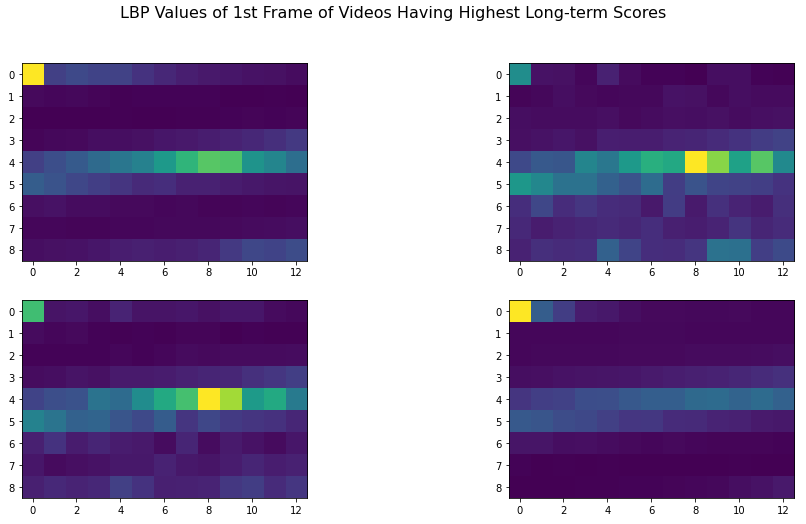
\includegraphics[width=\linewidth]{figures/high-long-memo-lbp.png}}
    \caption{The first frame's LBP of videos with the highest long-term memorability}
    \label{fig:high-long-memo-lbp}
\end{figure}

\begin{figure}[htbp]
    \centerline{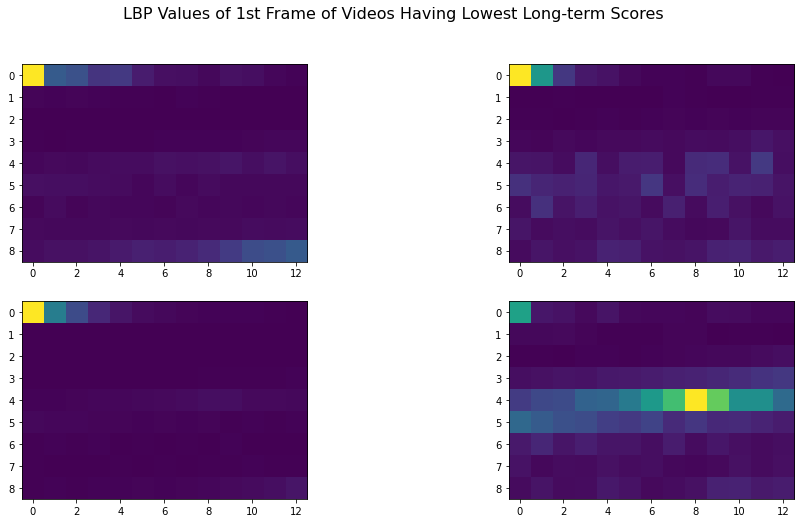
\includegraphics[width=\linewidth]{figures/low-long-memo-lbp.png}}
    \caption{The first frame's LBP of videos with the lowest long-term memorability}
    \label{fig:low-long-memo-lbp}
\end{figure}

\subsection{Using Principal Component Analysis on HMP}
Considering that the dimension of HMP was larger than the number of training samples, I conducted a Principal Component Analysis (PCA) on HMP to reduce its dimension.
The ratio of explained variance was $99.99\%$ if I kept the most 1000 critical dimensions.
Fig.~\ref{fig:pca-short-spearman-scores} shows the comparison of Spearman's scores for short-term predictions using only HMP in two cases with and without the PCA.

\begin{figure}[htbp]
    \centerline{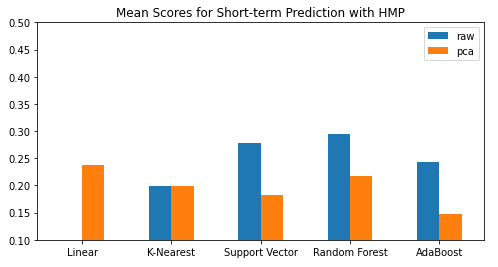
\includegraphics[width=\linewidth]{figures/pca-short-spearman-scores.png}}
    \caption{Spearman's scores for short-term predictions with only HMP}
    \label{fig:pca-short-spearman-scores}
\end{figure}

PCA only provided a significant performance improvement for Linear Regression.
For $K$-Nearest Neighbors Regression, it helped nothing.
To make matters worse, PCA reduced the prediction effect of the other three models.


\section{CONCLUSION AND FUTURE WORK}
I trained five different models with three features and their combinations, and compared the performance by Spearman's correlation coefficients.
For both short-term and long-term predictions, Random Forest Regression had the best result.
But the features were not the same.
For the short-term, the feature was C3D + HMP.
While for the long-term, it was C3D + LBP.

From the distribution of Random Forest feature importance, we can see that C3D provides much help for both types of predictions.
The short-term performance of the combination of C3D and HMP is better than using C3D alone, but HMP does not have high importance.
For LBP in long-term predictions, its values at the beginning, middle and end of a frame are more critical than others.
Memorable videos tend to have large LBP values at the middle of a frame.

In this paper, I only used three features, but MediaEval 2018 also provides other features such as color histograms.
In addition, I did not analyze why the 21st value of C3D is significantly more important than others for short-term predictions.
It may involve the structure of 3D Convolutional Networks.
From the aspect of models, only traditional machine learning algorithms had been tested. Deep Learning might be a good attempt.


\bibliographystyle{IEEEtranN}
\bibliography{media-memorability-prediction}

\end{document}